\section{Data Warehouse, Modelling, and Orchestration}

Once raw events land in Snowflake's \texttt{STAGING} schema, two additional layers convert them
into analytics-ready models: dbt handles the transformation logic,
and Airflow schedules the daily refresh.

\subsection{Star Schema with dbt}

dbt (data build tool) runs SQL transformations \emph{inside} Snowflake using the ELT pattern —
data is loaded first, then transformed in place, leveraging Snowflake's elastic compute.

\begin{figure}[H]
  \centering
  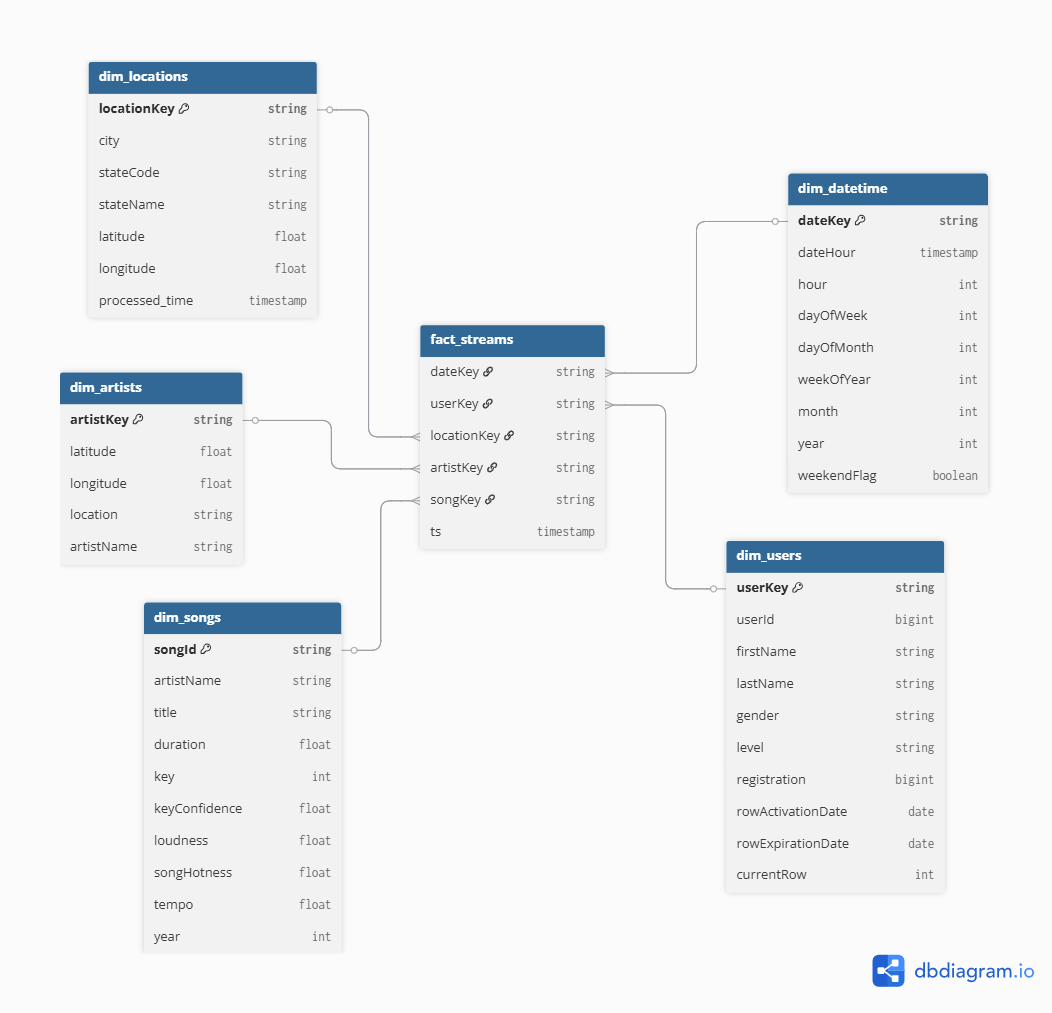
\includegraphics[width=0.88\textwidth]{../image/star_schema.png}
  \caption{Star schema produced by dbt: one fact table and five dimension tables.}
  \label{fig:star-schema}
\end{figure}

The dbt project produces two model layers:

\begin{itemize}
  \item \textbf{Star schema} — a normalised, storage-efficient structure optimised for data integrity:
    \begin{itemize}
      \item \texttt{fact\_streams} — the central fact table containing one row per song play, with foreign keys to all five dimensions.
      \item \texttt{dim\_users} — user demographics and subscription level.
      \item \texttt{dim\_songs} — track metadata (title, duration, artist reference).
      \item \texttt{dim\_artists} — artist name and location.
      \item \texttt{dim\_locations} — city, state, and geographic coordinates.
      \item \texttt{dim\_datetime} — date/time hierarchy (year, month, day, hour, weekday) for time-series drill-downs.
    \end{itemize}

  \item \textbf{Wide table} (\texttt{wide\_streams}) — a denormalised view built by pre-joining
        \texttt{fact\_streams} with all five dimension tables.
        It exists solely to simplify BI tool queries: Power BI users access a single flat table
        without needing to understand the underlying schema or write JOIN logic.
\end{itemize}

\begin{figure}[H]
  \centering
  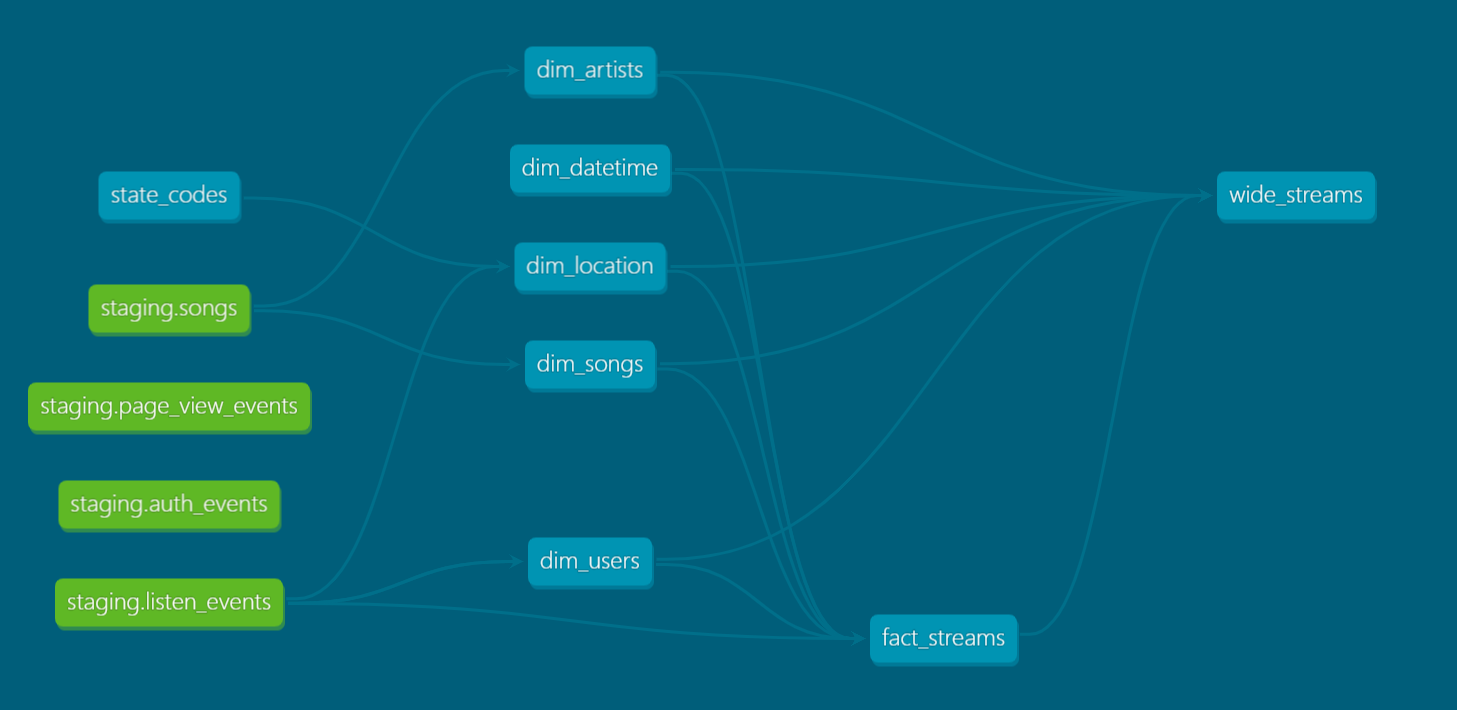
\includegraphics[width=0.85\textwidth]{../image/dbt_graph.png}
  \caption{dbt lineage graph: staging models feed into dimension and fact models, which feed the wide table.}
  \label{fig:dbt-graph}
\end{figure}

\subsection{Orchestration with Apache Airflow}

The Airflow DAG (\texttt{airflow/dags/dbt.py}) runs on a \textbf{daily schedule} and contains a
single task: a \texttt{DockerOperator} that spins up the official
\texttt{ghcr.io/dbt-labs/dbt-snowflake} container and executes \texttt{dbt run}
against the Snowflake warehouse.

Key design choices:
\begin{itemize}
  \item \textbf{Docker isolation} — dbt runs in its own container with mounted project and
        profile volumes, keeping the Airflow worker environment clean and the dbt version pinned.
  \item \textbf{Network sharing} — the container joins the \texttt{streamify\_my-network} Docker
        network, allowing it to reach the Snowflake JDBC endpoint.
  \item \textbf{Auto-remove} — the container is removed on success
        (\texttt{auto\_remove='success'}), preventing accumulation of stopped containers.
\end{itemize}

The Airflow web UI is available at \texttt{http://localhost:8000}.
